\subsection{7 Sites Results}

The 3 site case, although based on a real system currently functioning,
already contains a pooling effect due to the fact that some sites have more than one
machines. We would like to isolate the impact of just diversions in creating
the pooling effect. Thus,
it makes sense to conduct experiments on the case where instead of
having some big sites and some small sites, we have 7 small sites, each
with one machine. This system has worse performance initially
because no pooling effect is present. We shall examine the
impact of diversions. Note that all sites are totally homogeneous now:
they have the same number of machines, the same amount of load and
the same opening time. As a result, we do not need to look at system
performance at a per site level.

\begin{figure}[htp]
\centering
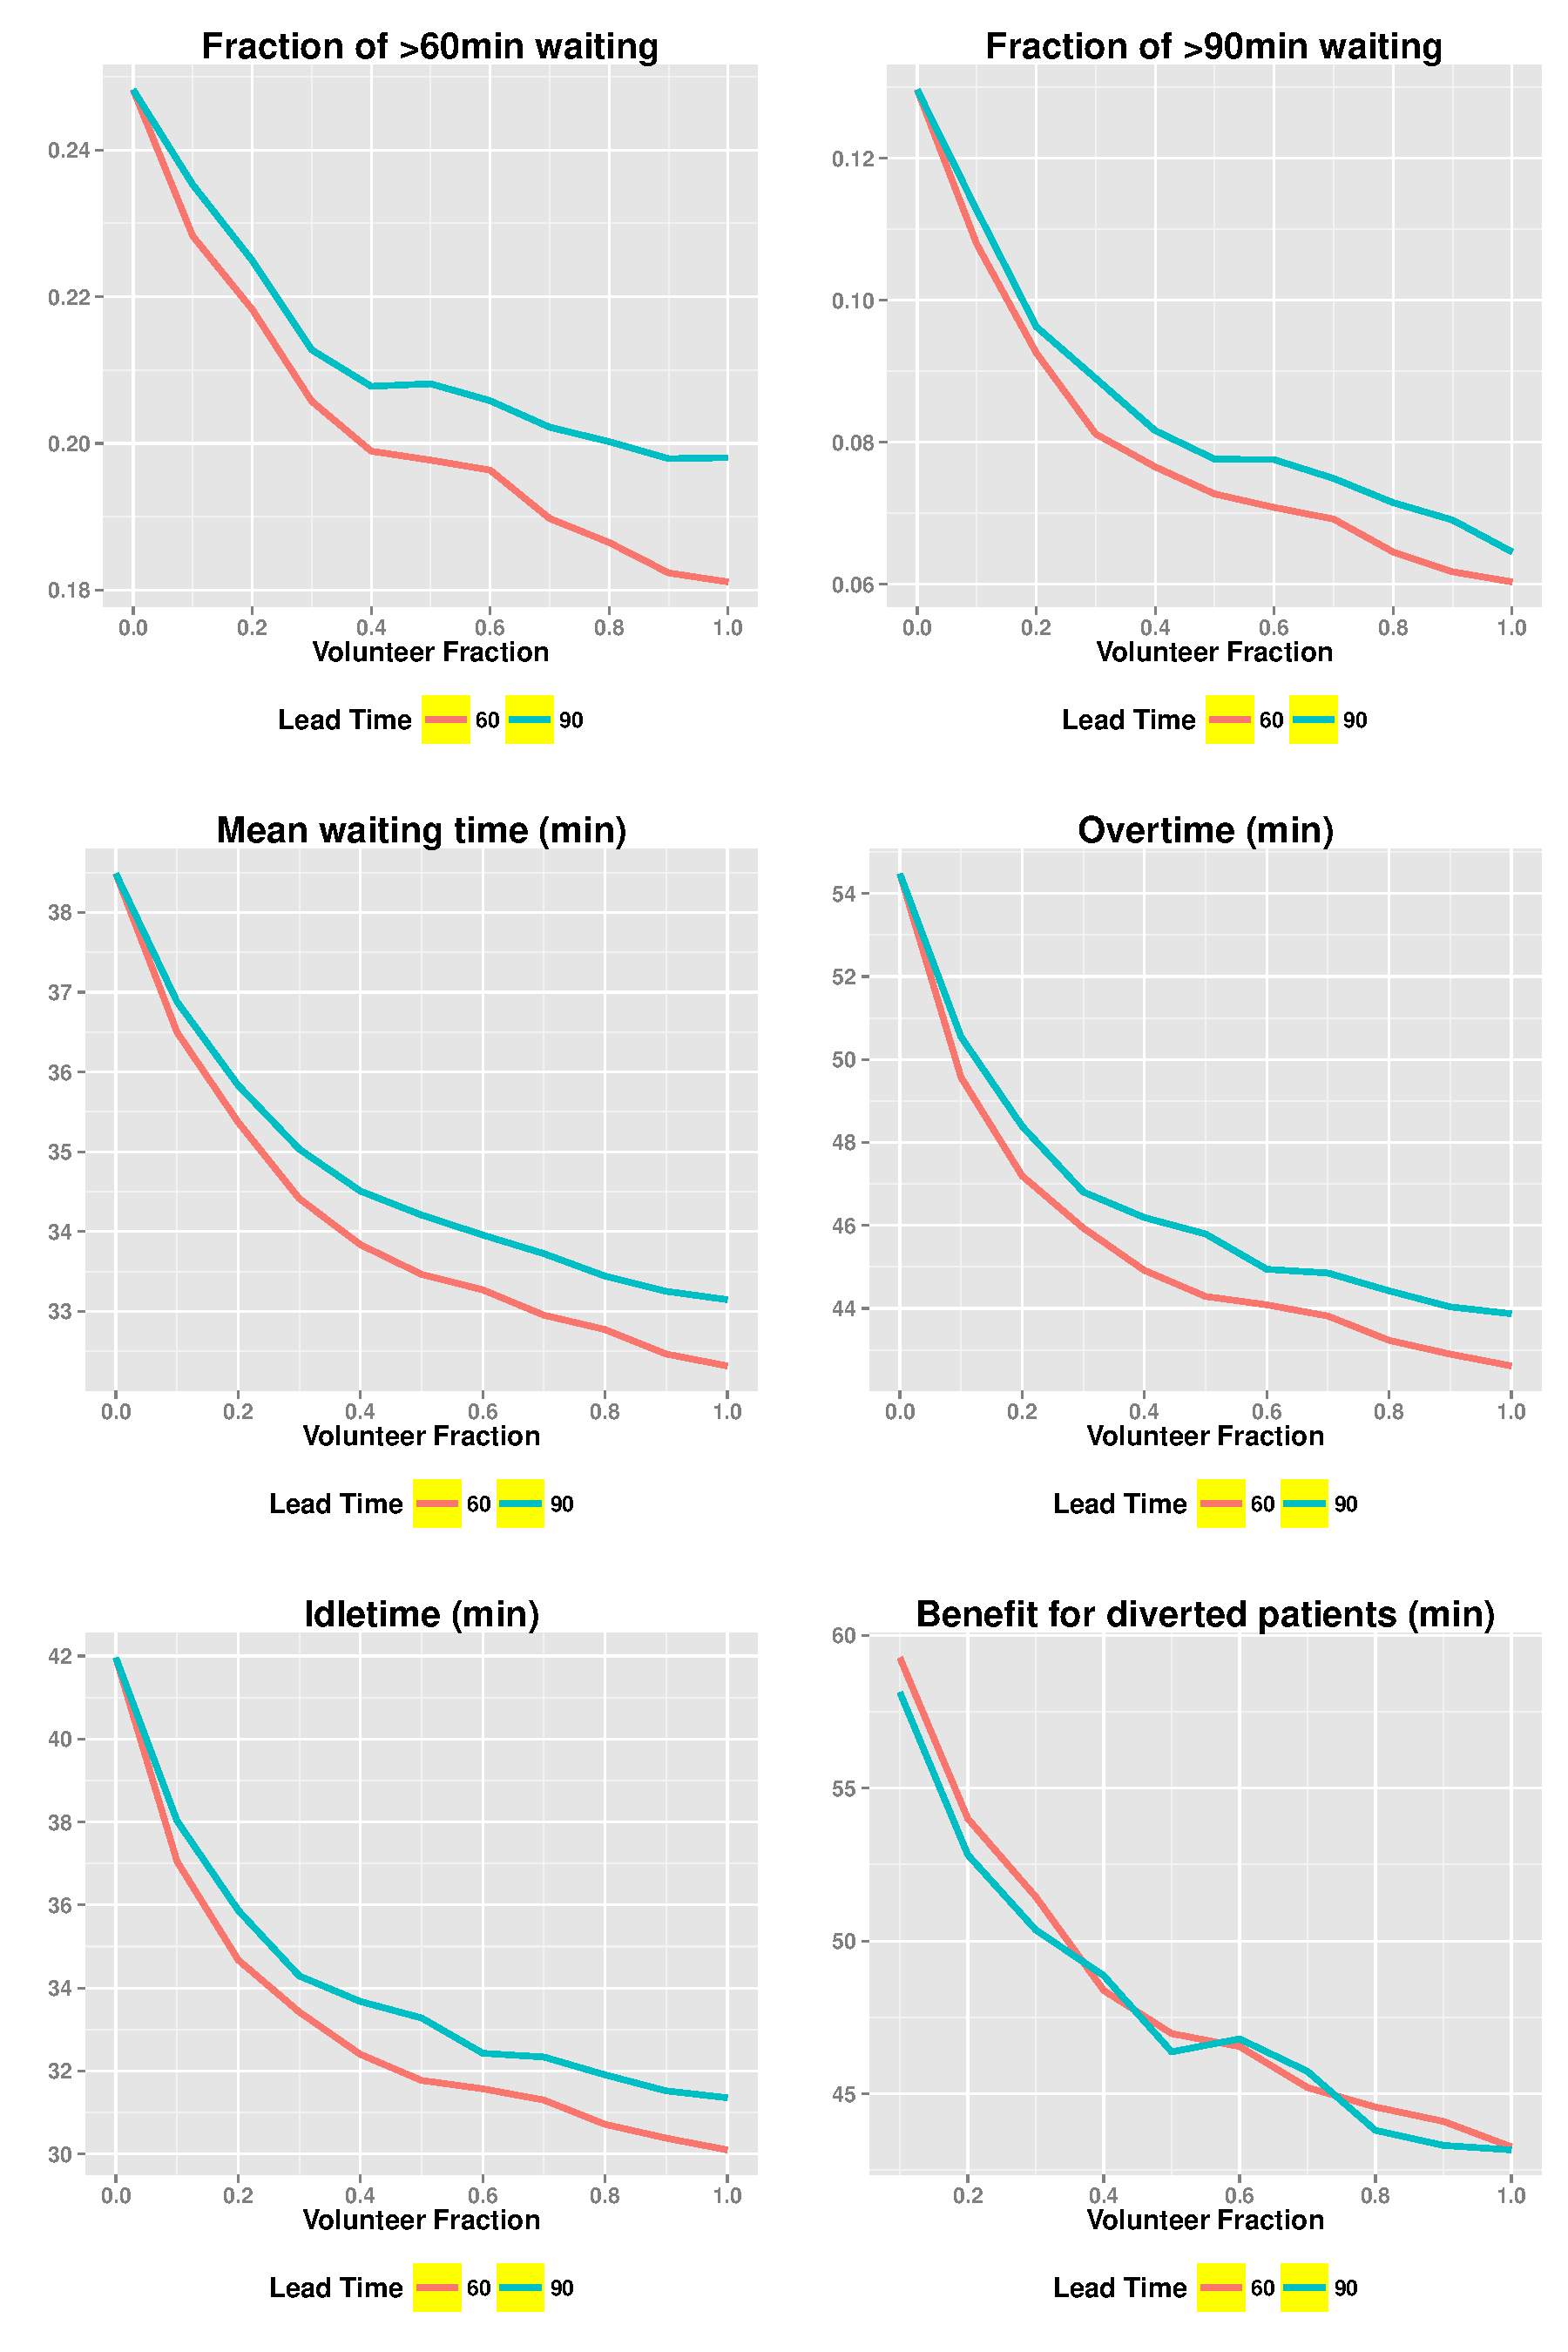
\includegraphics[width=.96\textwidth]{chap3/numeric/pic/7sites_all}
\caption{The impact of diversions on system performance of a system
with 7 sites, each with one machine.}
\label{fig:7sites_all}
\end{figure}

Figure \ref{fig:7sites_all} shows that when compared to 3 sites case,
diversions have a greater impact on this system. In this case, we have
significant improvement even on mean waiting time. This is exactly
because diversions provide the only source of a pooling effect.

\begin{figure}[htp]
\centering
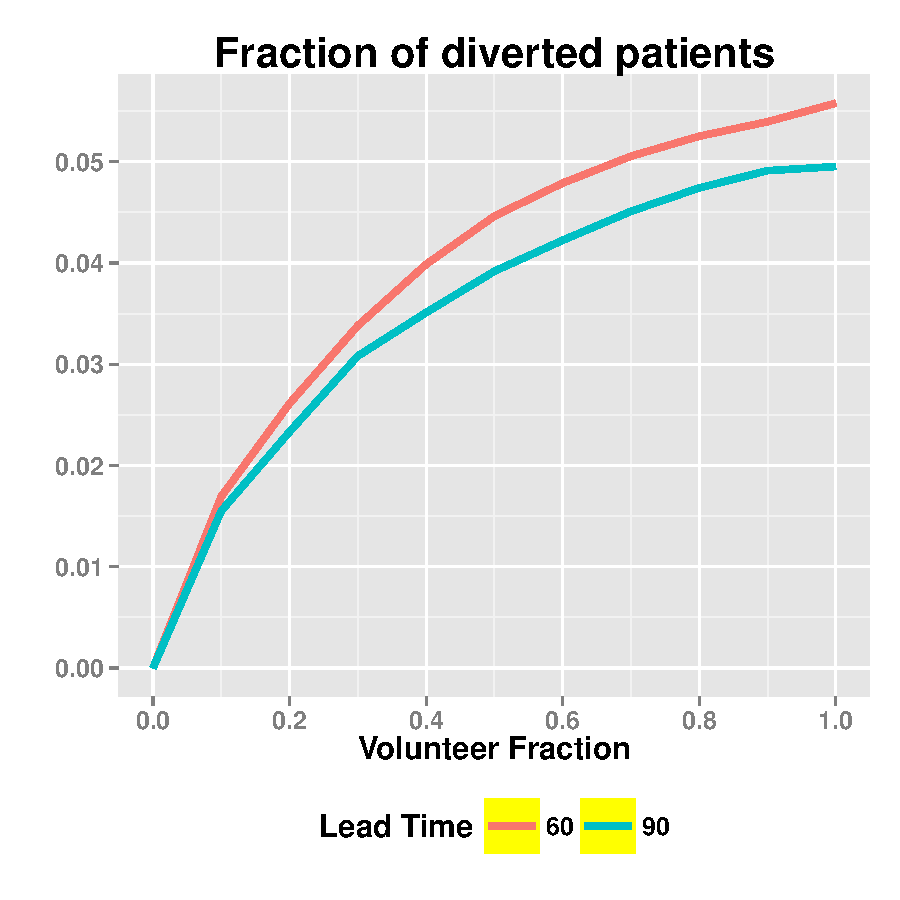
\includegraphics[width=.6\textwidth]{chap3/numeric/pic/7sites_all_diversion}
\caption{Fraction of diverted patients in 7 sites case.}
\label{fig:7sites_all_diversion}
\end{figure}

From Figure \ref{fig:7sites_all_diversion}, we see that we may potentially
divert 6\% patients if everyone volunteers. This is substantially more when compared
with 3 sites case. This shows that there are many more
beneficial diversion opportunities when there is no pooling initially. Also, for
diverted patients, each of them enjoys a greater reduction in waiting time
when compared to the 3 sites case.
